% % % % % % % % % % % % % % % % % % % % % % % % % % % % % % % % % % % % % % % % % % % %
%                                                                                     %
% Short Sectioned Assignment LaTeX Template Version 1.0 (5/5/12)                      %
% This template has been downloaded from: http://www.LaTeXTemplates.com               %
%                                                                                     %
% Original author:  Frits Wenneker (http://www.howtotex.com)                          %
%                                                                                     %
% Modified by: Fco Javier Sueza Rodríguez (fcosueza@disroot.org)                      %
%                                                                                     %
% Changes:                                                                            %
%	    - Custom Chapters, Sections and Subsections (titlesec package)                %
%           - Document type scrbook (oneside)                                         %
%           - Use babel-lang-spanish package and marvosym                             %
%           - Use hyperref, enumitem, tcolorbox and glossaries packages               %
%           - Use Time New Roman (mathptmx), Helvetic and Courier fonts               %
%                                                                                     %
% License: CC BY-NC-SA 3.0 (http://creativecommons.org/licenses/by-nc-sa/3.0/)        %
%                                                                                     %
% % % % % % % % % % % % % % % % % % % % % % % % % % % % % % % % % % % % % % % % % % % %

%-----------------------------------------------%
%	              Packages                  %
%-----------------------------------------------%

\documentclass[paper=a4, fontsize=11pt, oneside]{scrbook}

% ---- Text Input/Output ----- %

\usepackage[T1]{fontenc}
\usepackage[utf8]{inputenc}
\usepackage{mathptmx}
\usepackage[scaled=.92]{helvet}
\usepackage{courier}
\usepackage[indent=12pt]{parskip}

\usepackage{geometry}
\geometry{verbose,tmargin=3cm,bmargin=3cm,lmargin=2.6cm,rmargin=2.6cm}

% ---- Language ----- %

\usepackage[spanish]{babel}
\usepackage{marvosym}

% ---- Another packages ---- %

\usepackage{amsmath,amsfonts,amsthm}
\usepackage{graphics,graphicx}
\usepackage{titlesec}
\usepackage{fancyhdr}
\usepackage{tcolorbox}
\usepackage{hyperref}
\usepackage{enumitem}
\usepackage[automake]{glossaries}

%--------------------------------------------------------------------%
%                      Customizing Document                          %
%--------------------------------------------------------------------%


% ----------- Custom Chapters, Sections and Subsections -------------- %

\titleformat{\chapter}[display]
			{\bfseries\Huge}
			{Tema \ \thechapter} {0.5ex}
			{\vspace{1ex}\centering}

\titleformat{\section}[hang]
			{\bfseries\Large}
			{\thesection}{0.5em}{}

\titleformat{\subsection}[hang]
			{\bfseries\large}
			{\thesubsection}{0.5em}{}

\titleformat{\subsubsection}[hang]
			{\bfseries\large}
			{\thesubsubsection}{0.5em}{}

\hypersetup{
    colorlinks=true,
    linkcolor=black,
    urlcolor=magenta
}

% ------------------- Custom heaaders and footers ------------------- %

\pagestyle{fancyplain}

\fancyhead[]{}
\fancyfoot[L]{}
\fancyfoot[C]{}
\fancyfoot[R]{\thepage}

\renewcommand{\headrulewidth}{0pt} % Remove header underlines
\renewcommand{\footrulewidth}{0pt} % Remove footer underlines

\setlength{\headheight}{13.6pt} % Customize the height of the header

% --------- Numbering equations, figures and tables ----------------- %

\numberwithin{equation}{section} % Number equations within sections
\numberwithin{figure}{section} % Number figures within sections
\numberwithin{table}{section} % Number tables within sections

% ------------------------ New Commands ----------------------------- %

\newcommand{\horrule}[1]{\rule{\linewidth}{#1}} % Create horizontal rule command


%----------------------------------------------------------------------------------------
%	TÍTULO Y DATOS DEL ALUMNO
%----------------------------------------------------------------------------------------

\title{
\vspace{10ex}
\normalfont \normalsize
\Huge \textbf{Tarea 3: Análisis y Diseño de Redes}
}
\author{Francisco Javier Sueza Rodríguez}
\date{\normalsize\today}

%----------------------------------------------------------------------------------------
%                                     DOCUMENTO
%----------------------------------------------------------------------------------------
\begin{document}

\maketitle

\thispagestyle{empty}

\vspace{68ex}

\begin{center}
    \begin{tabular}{l l}
        \textbf{Centro}: & IES Aguadulce \\
        \textbf{Ciclo Formativo}: & Desarrollo Aplicaciones Web (Distancia)\\
        \textbf{Asignatura}: & Sistemas Informáticos\\
        \textbf{Tema}: & Tema 3 -  Redes de Ordenadores\\
    \end{tabular}
\end{center}

\newpage

\tableofcontents

\vspace{15ex}

\hrule

\vspace{10ex}

\listoffigures

\newpage

\section{Caso Práctico}
Antonio y Juan han sido nombrados responsables del área de sistemas y redes de la nueva empresa AguadulSoft.

La semana pasada tuvieron una reunión con Ada en la que se les comunicó que tendrían que encargarse de proyectos de implantación de redes en oficinas de clientes. Su primer trabajo será un proyecto pequeño para una biblioteca/centro lúdico de una pequeña población cercana. Antes de lanzarse a dicha tarea van a repasar algunos conceptos básicos de redes.

\section{Actividades}

\subsection{Actividad 1: Medios de Trans}

\subsubsection{Enunciado}

Para esta actividad debes realizar dos tablas con información obtenida en Internet o en los contenidos de la unidad sobre los siguientes medios de transmisión:misión

\subsubsection*{Parte A: Medios Guiados}
Recientemente, el estándar cableado Ethernet de 2.5 Gbps sobre cable de par trenzado está ganando popularidad. Buscando información en Internet, haz una tabla que incluya lo siguiente:

\begin{figure}[H]
    \centering
    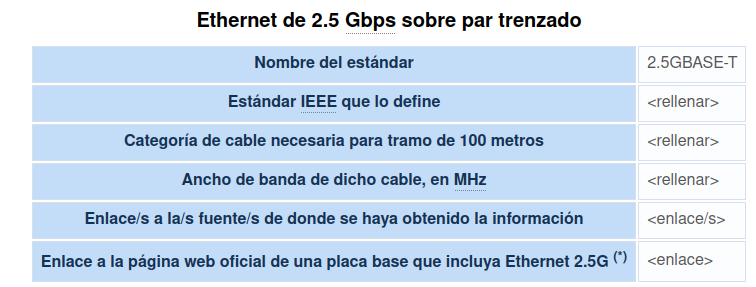
\includegraphics[scale=0.42]{tabla-eth.png}
    \caption{Tabla a completar con datos de la interfaz Ethernet}
\end{figure}

\subsubsection*{Parte B: Medios inalámbricos}
En cuanto a medios inalámbricos, la tecnología que se está implantando en mayor medida en la actualidad es Wi-Fi 6. Busca información en Internet o en los contenidos de la unidad y rellena una tabla como la siguiente:

\begin{figure}[H]
    \centering
    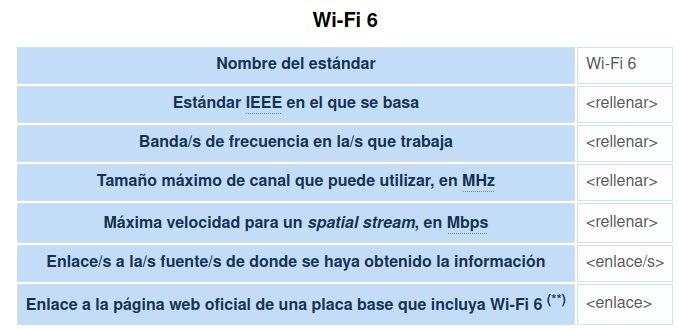
\includegraphics[scale=0.42]{tabla-wifi.png}
    \caption{Tabla a completar con datos de la interfaz Wifi}
\end{figure}

\subsubsection{Respuesta}

\subsubsection*{Parte 1: Medios Guiados}
En primer lugar vamos a rellenar la tabla con las especificaciones del estándar Ethernet 2.5 Gbs, la información sobre este estándar la hemos recogido de la página de wikipedia \cite{wiki01}, ya que la versión del estándar en la web del IEEE es de pago.

La tabla a quedado así:

\begin{figure}[H]

    \vspace{3ex}
    \centering

    \setlength{\tabcolsep}{10pt}
    \renewcommand{\arraystretch}{1.4}

    \begin{tabular}{| l | l |}
        \hline
        \textbf{Nombre del estándar}  & 2.5GBASE-T \\ \hline
        \textbf{Estándar IEEE que lo define} & IEEE 802.3bz   \\ \hline
        \textbf{Categoría de cable necesaria para tramo de 100 metros} & Cat 5e   \\ \hline
        \textbf{Ancho de banda de dicho cable} & 100 MHz    \\ \hline
        \textbf{Enlace/s a la/s fuente/s} & \href{https://es.wikipedia.org/wiki/IEEE_802.3bz_(2.5GBASE-T_y_5GBASE-T)}{Wikipedia IEEE 802.3bz}  \\ \hline
        \textbf{Placa Base que incluye Ethernet 2.5G} & \href{https://www.gigabyte.com/Motherboard/Z790-AORUS-XTREME-rev-10/sp#sp}{Gigabyte Z790 AORUS Extreme}   \\ \hline
    \end{tabular}
    \caption{Tabla: Características estándar Ethernet 2.5G}
\end{figure}

\subsubsection*{Parte 2: Medios inalámbricos}
En esta segunda parte vamos a rellenar la tabla con las características del estándar Wifi 6. La información, igual que en el punto anterior, ha sido extraído de la página de Wikipedia relativa al estándar Wifi 6 \cite{wiki02} y la tabla a quedado de la siguiente forma:

\begin{figure}[H]

    \vspace{3ex}
    \centering

    \setlength{\tabcolsep}{10pt}
    \renewcommand{\arraystretch}{1.4}

    \begin{tabular}{| l | l |}
        \hline
        \textbf{Nombre del estándar}  & Wifi 6 \\ \hline
        \textbf{Estándar IEEE que lo define} & IEEE 802.11ax   \\ \hline
        \textbf{Banda/s de frecuencia en la/s que trabaja} & 2.5GHz, 5GHz y 6GHz \\ \hline
        \textbf{Tamaño máximo de canal que puede utilizar, en MHz} & 160 MHz    \\ \hline
        \textbf{Máxima velocidad para un spatial stream, en Mbps} & 1201 Mbps \\ \hline
        \textbf{Enlace/s a la/s fuente/s} & \href{https://en.wikipedia.org/wiki/Wi-Fi_6}{Wikipedia Wifi 6}  \\ \hline
        \textbf{Placa Base que incluye Wifi 6} & \href{https://www.gigabyte.com/Motherboard/Z790-AORUS-XTREME-rev-10/sp#sp}{Gigabyte Z790 AORUS Extreme}   \\ \hline
    \end{tabular}
    \caption{Tabla: Características estándar Wifi 6}
\end{figure}

\subsection{Actividad 2: Conociendo mi equipo de Interconexión}

\subsubsection{Enunciado}
Para esta actividad vas a intentar analizar el router casero que proporciona conexión a Internet en tu casa. Realiza una fotografía al router de tu casa por las partes donde se encuentren los puertos de conexión, botones y cableado, con cuidado de no mostrar información sensible como contraseñas. Si el dispositivo tiene botones frontales, muéstralos también. En dicha fotografía señala todos los botones, puertos y elementos que veas, márcalos con un número cada uno, y haz una tabla en la que indiques:

\begin{figure}[H]
    \centering
    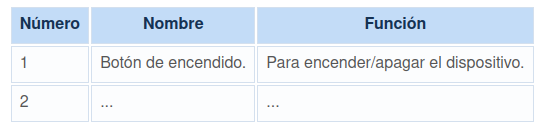
\includegraphics[scale=0.55]{tabla-router.png}
    \caption{Tabla a rellenar sobre el router}
\end{figure}

A continuación, contesta a las siguientes preguntas acerca de tu router ISP:

\begin{itemize}
    \item ¿Qué tipo de conexión a Internet proporciona y qué tipo de cableado usa para la conectividad WAN externa? (fibra óptica, DOCSIS con cable coaxial, ADSL con par trenzado telefónico, cable de par trenzado a una ONT externa...)
    \item ¿Realiza la función de ``conmutador'' (switch)? ¿Cuántos puertos conmutados tiene? ¿En qué consiste dicha función?
    \item ¿Realiza la función de ``punto de acceso inalámbrico''? ¿En qué consiste dicha función?
    \item ¿Realiza la función de ``servidor DHCP''? ¿En qué consiste dicha función?
\end{itemize}

\subsubsection{Respuesta}
En primer lugar, vamos a mostrar una imagen, tanto frontal como trasera del router, especificando las diferentes conexiones y botones que tiene el router. En concreto, el router es un modelo \textbf{Sagemcom Fast 5657} y las imágenes son las siguientes:

    \begin{figure}[H]
    \centering
    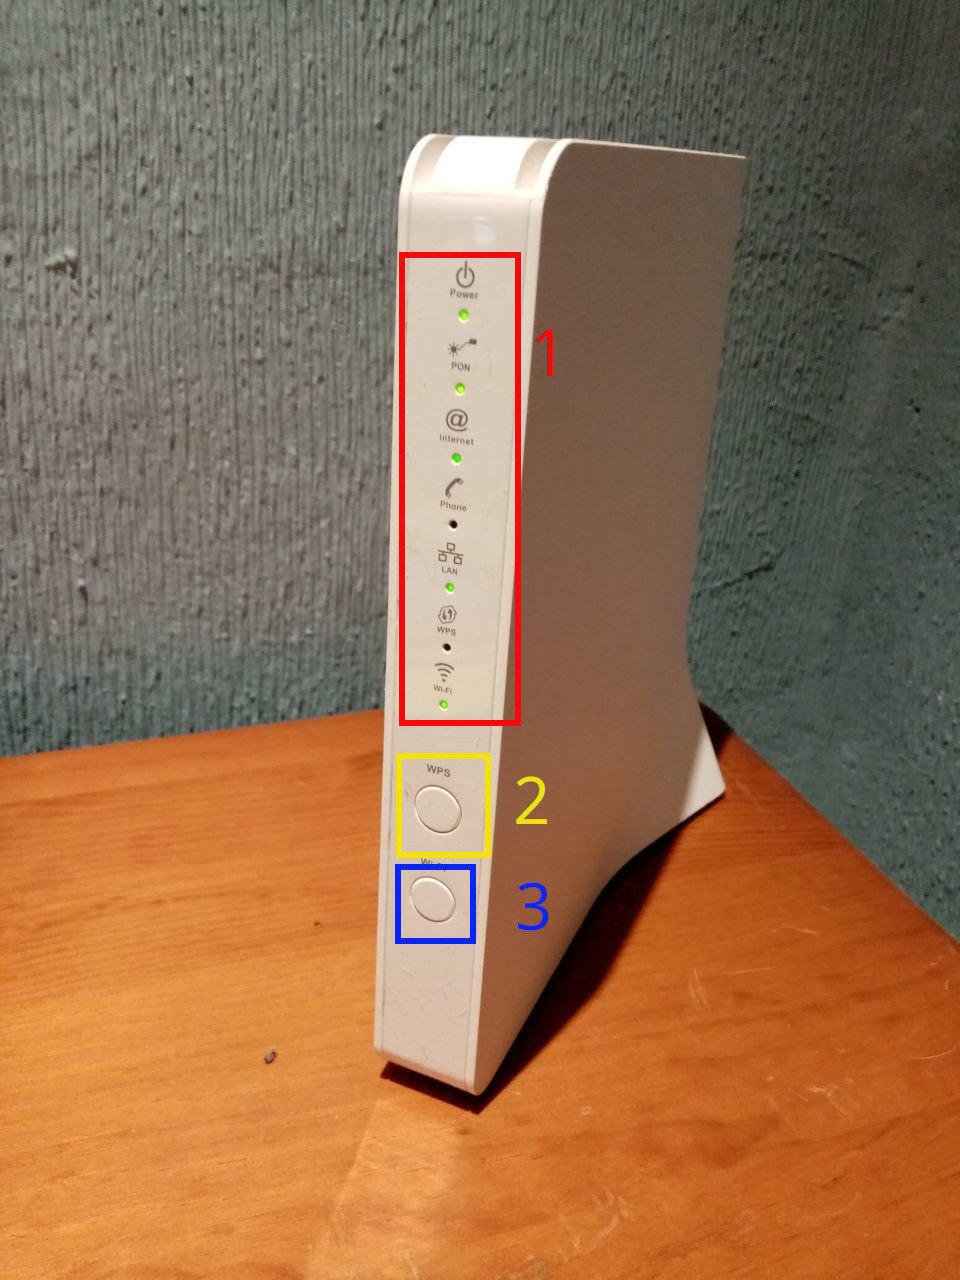
\includegraphics[scale=0.85]{router-delantera.jpg} \hspace{3ex}
    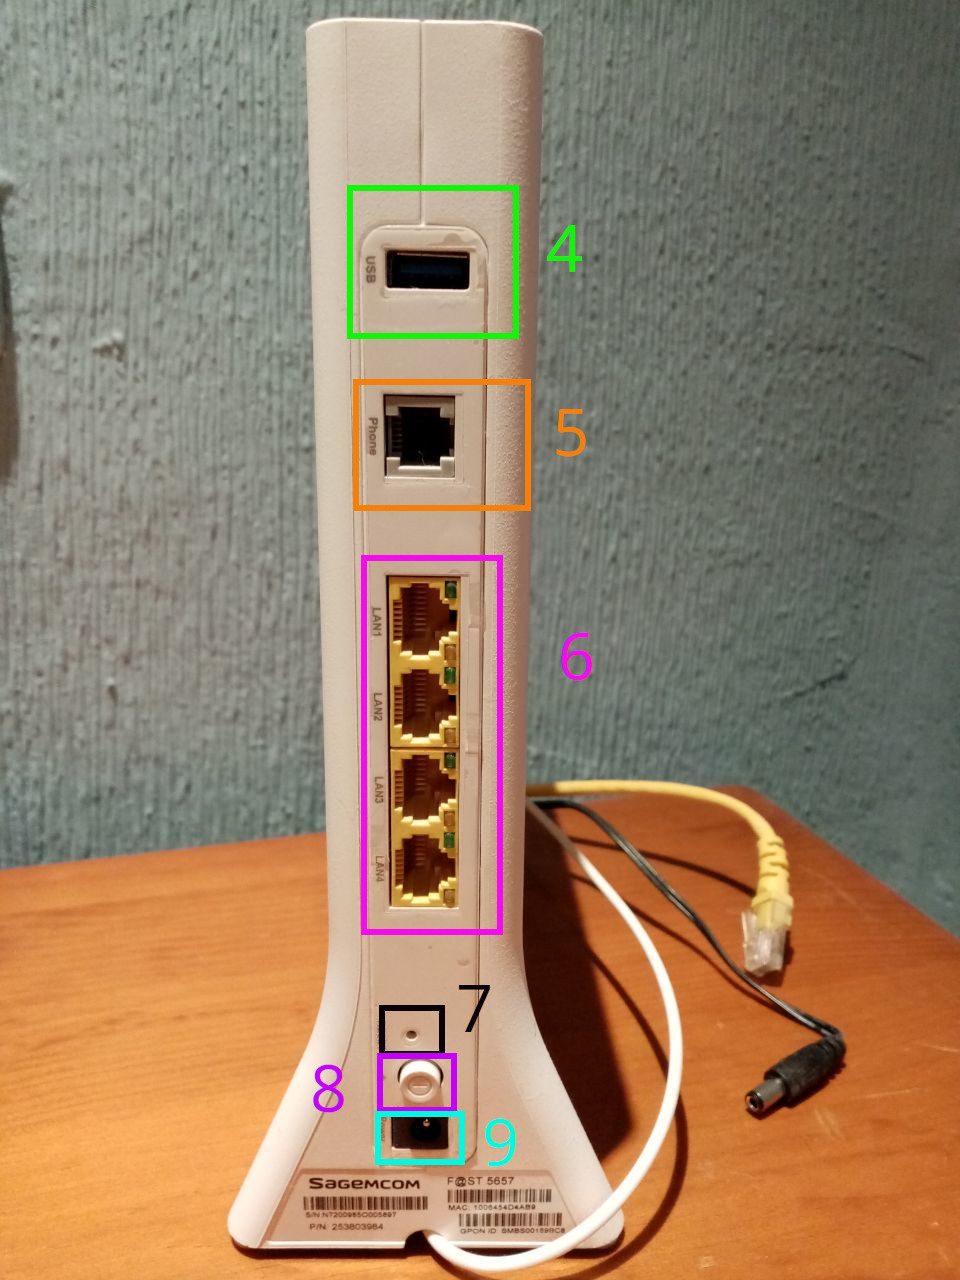
\includegraphics[scale=0.85]{router-trasera.jpg}
    \caption{Imagen delantera y trasera del router}
\end{figure}

A continuación de muestra la tabla con la funcionalidad de cada uno de los elementos señalados en las imágenes:

    \begin{figure}[H]

    \vspace{3ex}
    \centering

    \setlength{\tabcolsep}{10pt}
    \renewcommand{\arraystretch}{1.4}

    \begin{tabular}{| m{4em} | m{13em} | m{17em} |}
        \hline
        \textbf{Número}  & \textbf{Nombre} & \textbf{Función} \\ \hline
        \centering 1 &  LEDs de Estado & Estos LED indican el estado de las diferentes conexiones \\ \hline
        \centering 2 &  Botón WPS & Este botón habilita la función WPS del router, que permite la conexión segura de dispositivos sin utilizar la contraseña de red, usando en su defecto, por ejemplo, un número PIN \\ \hline
        \centering 3 &  Botón Wifi & Este botón sirve para habilitar o deshabilitar las redes Wifi, tanto la 2.4 Ghz como la de 5Ghz, básicamente deshabilita la funcionalidad Wifi del router. \\ \hline
        \centering 4 &  Puerto USB & Sirve para conectar dispositivos USB, en concreto, dispositivos de almacenamiento, ta que el router tiene la capacidad de servirlos mediante un servidor FTP. \\ \hline
        \centering 5 &  Puerto de Telefono & Conexión de tipo RJ-11  que nos permite conectar une teléfono fijo al router\\ \hline
        \centering 6 &  Puertos LAN & Son 4 conexiones de tipo RJ-45 que nos permiten conectar hasta 4 dispositivos al router de forma cableada. \\ \hline
        \centering 7 &  Botón de reset & Botón que nos permite resetear el router a la configuración que trae por defecto de fábrica \\ \hline
        \centering 8 &  Botón de Encendido/Apagado & Botón que nos permite encender y apagar el router \\ \hline
        \centering 9 &  Conexión de Energía & Clavija que nos permite conectar el cable de alimentación del router \\ \hline
    \end{tabular}
    \caption{Tabla de elementos externos del router}
\end{figure}

Respecto a las preguntas del enunciado, las respuestas son las siguientes:

\begin{itemize}
    \item El router proporciona conexión tanto \textbf{cableada} como \textbf{inalámbrica}, y tiene un cableado para la conexión WAN de \textbf{fibra óptica}.
    \item Ha sido complicado encontrar información sobre el router y sus características, aunque después de visitar varias páginas de internet y navegar por la configuración del router, he llegado a la conclusión de que \textbf{no ofrece la función} de \textbf{conmutador}. Aún así, se puede ``configurar'' para que realice dicha función deshabilitando diferentes opciones y editando la tabla de rutas, pero no incorpora la función de forma nativa, por lo que \textbf{no tiene puertos conmutados}.

    Esta \textbf{función}, como hemos visto en el tema, se encarga de \textbf{conectar varios ordenadores}, de forma rápida y eficiente, mediante el \textbf{almacenamiento de las direcciones MAC} de los dispositivos conectados a él. Esta función, pertenece a la\textbf{ capa 2 del nivel OSI} o \textbf{nivel de enlace de datos}.

    \item Este router \textbf{si realiza de función} de \textbf{punto de acceso inalámbrico}.

    Esta \textbf{función} la realiza un dispositivo que permite la conexión de dispositivos de forma inalámbrica a la red, permitiéndoles el acceso tanto a internet como a la red local.

    \item Este router \textbf{si realiza la función} de \textbf{servidor DHCP}.

    El \textbf{servidor DHCP}, como hemos visto en el tema, se encarga de la asignación de direcciones IP, la cual se puede hacer de forma \textbf{dinámica} o \textbf{reservando} las direcciones IP. Además, se encarga de la información de la configuración de red en general.
\end{itemize}


\subsection{Actividad 3: Interpretar un diagrama de red lógico y componentes de una red}

\subsubsection{Enunciado}
Supongamos que tenemos una red correspondiente a la oficina de la empresa AguadulSoft, como la que se representa en el siguiente diagrama de red lógico. En esta red hay unos despachos en los que se sitúan un servidor de archivos y seis equipos, y un aula de formación donde hay veinte equipos fijos y la posibilidad de conectar otros dispositivos móviles de manera inalámbrica (pulsa la imagen para ampliarla).

\begin{figure}[H]
    \centering
    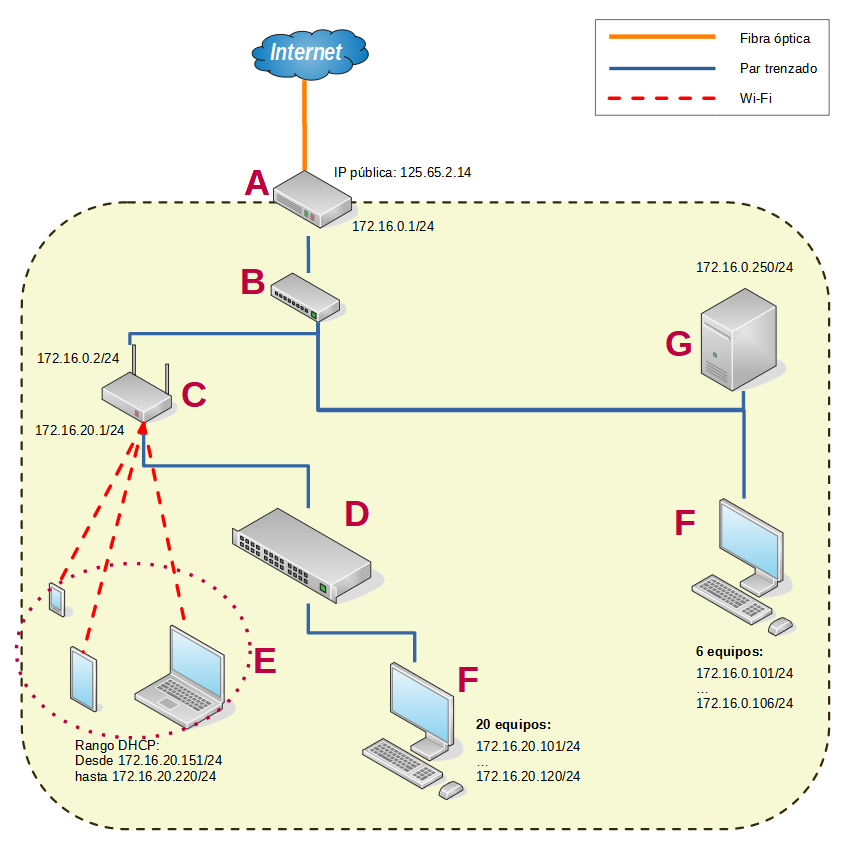
\includegraphics[scale=0.37]{red-logica.png}
    \caption{Diagrama de red lógico actividad 3}
\end{figure}

Realiza las siguientes tareas o contesta a las preguntas que se hacen en relación a la red que está englobada en el cuadro de color lima:

\begin{enumerate}
    \item Clasifica esta red según los siguientes criterios, razonando las respuestas (en los contenidos de la unidad están explicados estos criterios de clasificación de redes):
    \begin{itemize}
        \item Su extensión.
        \item Las funciones de sus componentes.
        \item El tipo de conexión.
    \end{itemize}

    \item Realiza una tabla en la que indiques la siguiente información relativa a cada uno de los elementos marcados con una letra mayúscula en el diagrama lógico:

    \begin{figure}[ht]
        \centering
        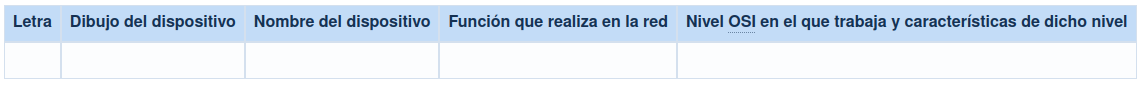
\includegraphics[scale=0.45]{tabla-red.png}
        \caption{Tabla elementos de red actividad 3}
    \end{figure}
\end{enumerate}

\subsubsection{Respuesta}

En primer lugar vamos a \textbf{clasificar la red} según los diferentes criterios que se nos han pedido, siendo los siguientes:

\begin{itemize}
    \item \textbf{Extensión}: estar red sería una red \textbf{LAN}, ya que todos los dispositivos se encuentran en un mismo edificio.

    \item \textbf{Funciones de sus componentes}: en este caso dependerá de que parte de la red analicemos, ya que en los \textbf{despachos} se podría considerar que la conexión es de tipo \textbf{cliente-servidor}, pero en la subred del \textbf{aula de formación} nos encontramos ante una red de tipo \textbf{peer-to-peer}.

   \item \textbf{Tipos de conexión}: estamos ante una \textbf{red mixta}, ya que nos encontramos equipos que se conectan mediante cable pero también hay posibilidad de que se conecten de forma inalámbrica.
\end{itemize}



% Bibliography

\newpage
\bibliography{citas}
\bibliographystyle{unsrt}

\end{document}